% !TeX root = euclid-without-words.tex
% !TeX Program=pdfLaTeX
%
% Diagonals of a kite
%
\begin{minipage}[t]{.48\textwidth}
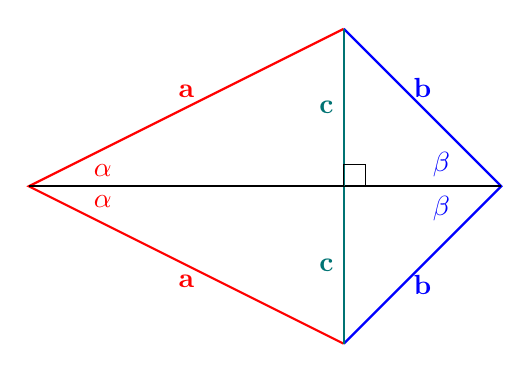
\begin{tikzpicture}[scale=1]
% Draw the kite
\coordinate (a) at (0,0);
\coordinate (b) at (4,2);
\coordinate (c) at (6,0);
\coordinate (d) at (4,-2);
\coordinate (intersection) at (4,0);
\draw[red,thick] (d) -- node[below] {$\mathbf{a}$} (a) -- node[above] {$\mathbf{a}$} (b);
\draw[blue,thick] (b) -- node[above] {$\mathbf{b}$} (c) -- node[below] {$\mathbf{b}$} (d);
% Label nodes
\node[red,above right,xshift=20pt] at (a) {$\bm{\alpha}$};
\node[red,below right,xshift=20pt] at (a) {$\bm{\alpha}$};
\node[blue,above left,xshift=-15pt] at (c) {$\mathbf{\beta}$};
\node[blue,below left,xshift=-15pt] at (c) {$\mathbf{\beta}$};
% Draw diagonals
\draw[thick] (a) -- (c);
\draw[black!10!teal,thick] (b) -- node[left] {$\mathbf{c}$}(intersection) -- node[left] {$\mathbf{c}$} (d);

% Draw square to denote right angle
\draw (intersection) rectangle +(8pt,8pt);
\end{tikzpicture}
\end{minipage}
